% =============================================================================
% REGRESSÃO DESCONTÍNUA (15:15 a 15:30)   [Script 05]
% =============================================================================
\section[RDD]{Regressão descontínua}
\subsection{Ideia e exemplos}

\begin{frame}{A ideia: um ``experimento natural'' no corte}
  \begin{itemize}
    \item Muitos programas têm uma \ind{regra de elegibilidade}: um índice contínuo e um \textbf{ponto de corte};
    \item Ex.: transferência de renda para quem tem renda per capita \textbf{até R\$ 77}. Uma família com R\$ 77 recebe; outra com R\$ 78, não;
    \item Perto do corte, as famílias são muito parecidas: é \destaque{como se houvesse um sorteio};
    \item O impacto é o tamanho do \ind{salto} no corte.
  \end{itemize}
\end{frame}

\begin{frame}{Regressão descontínua: características e exemplos}
  \carac{famílias \textbf{logo do outro lado do corte}}
        {\textbf{continuidade}: sem manipulação do corte e sem outros saltos no mesmo ponto}
        {efeito \textbf{local}, para quem está no corte}
        {índice contínuo, corte claro e \textbf{muitas observações} perto dele}
        {programas com elegibilidade por escore (renda, nota, idade, população)}
  \vspace{0.05cm}
  \textbf{\footnotesize\color{azul}Exemplos em políticas públicas}\par
    \scriptsize
    \begin{itemize}
      \item \textbf{México:} elegibilidade do Progresa e frequência escolar (Buddelmeyer e Skoufias, 2004).
      \item \textbf{Israel:} turmas divididas quando passam de 40 alunos (regra de Maimônides) e desempenho (Angrist e Lavy, 1999).
      \item \textbf{Eleições:} candidatos eleitos por margem mínima (Lee, 2008).
    \end{itemize}
\end{frame}

\begin{frame}{A descontinuidade no corte}
  \centering
  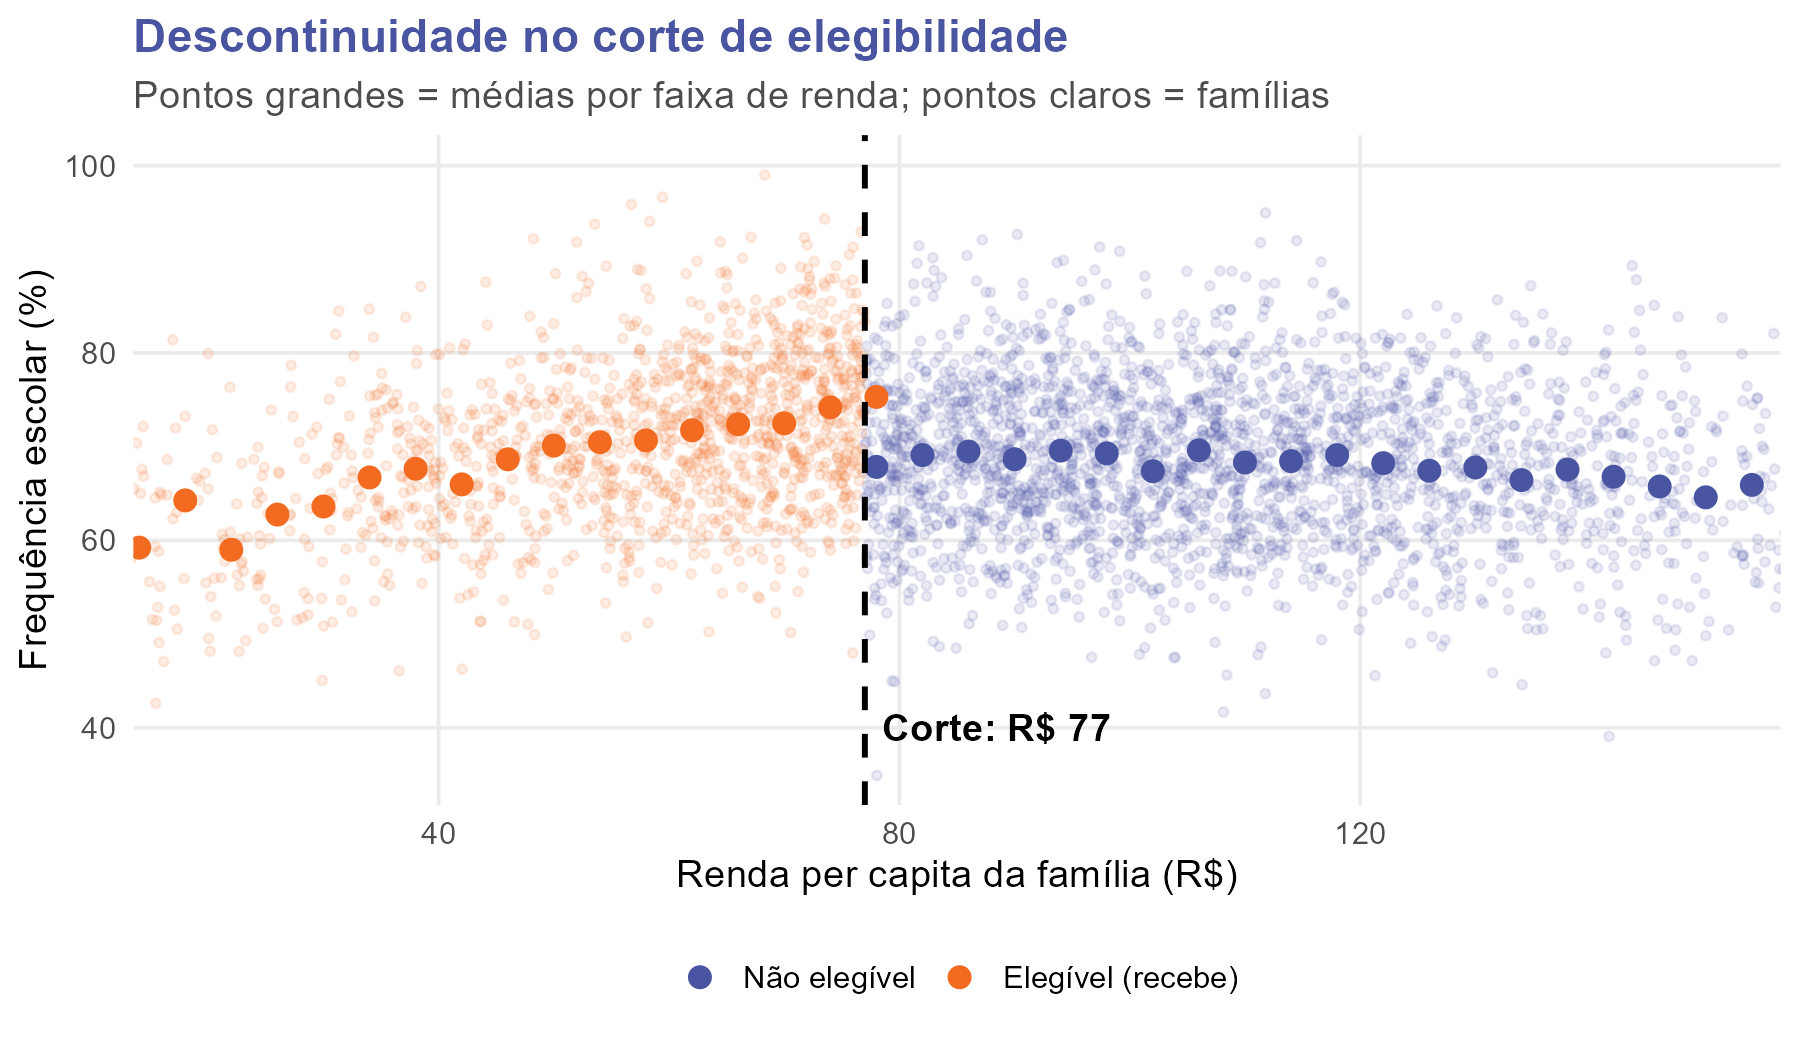
\includegraphics[height=4.2cm]{05_rdd_dispersao.png}\par
  \footnotesize Pontos grandes: médias por faixa de R\$ 4. Elegíveis (laranja) têm frequência escolar maior logo abaixo do corte.
\end{frame}

\subsection{Passo a passo}

\begin{frame}[fragile]{RDD, passo 1: de quanto é o salto no corte?}
\begin{consoleR}
@@> rd <- rdrobust(y = d$freq, x = -d$x)
@@> with(rd, round(data.frame(efeito = coef[1], ep = se[1],
@@+       ic_inf = ci[3, 1], ic_sup = ci[3, 2],
@@+       h = bws[1, 1]), 2))
  efeito   ep ic_inf ic_sup     h
1   6.75 0.93   5.03   9.19 16.78
\end{consoleR}
\begin{leitura}
  \begin{itemize}\setlength{\itemsep}{1pt}
    \item \rot{Onde olhar:} o \texttt{rdrobust} escolhe a janela sozinho (\texttt{h} $=16{,}8$) e estima o salto: \destaque{6,75 pontos} de frequência escolar (verdade: 6), EP 0,93. Usamos \texttt{x = -d\$x} porque os elegíveis estão \emph{abaixo} do corte.
    \item \rot{Corte:} IC robusto de 5,0 a 9,2, sem zero (Calonico, Cattaneo e Titiunik, 2014).
  \end{itemize}
\end{leitura}
\end{frame}

\begin{frame}[fragile]{RDD, passo 2: o resultado depende da janela?}
\begin{consoleRpeq}
@@> t(sapply(c(5, 15, 40), function(h) {
@@+   r <- rdrobust(d$freq, -d$x, h = h)
@@+   round(c(h = h, efeito = r$coef[1], ep = r$se[1],
@@+           controle = r$N_h[1], tratamento = r$N_h[2]), 2)
@@+ }))
      h efeito   ep controle tratamento
[1,]  5   7.21 1.59      227        213
[2,] 15   6.95 0.98      655        616
[3,] 40   5.79 0.64     1684       1149
\end{consoleRpeq}
\begin{leitura}
  \begin{itemize}\setlength{\itemsep}{1pt}
    \item \rot{Onde olhar:} \texttt{h} é a janela em R\$; \texttt{controle} e \texttt{tratamento} são as famílias de cada lado dentro dela. O efeito fica entre 5,8 e 7,2: não depende da janela.
    \item \rot{Corte:} mostrar várias janelas (Lee e Lemieux, 2010).
  \end{itemize}
\end{leitura}
\end{frame}

\begin{frame}[fragile]{RDD, passo 3: os dois lados do corte são comparáveis?}
\begin{consoleR}
@@> rc <- rdrobust(d$idade_mae, -d$x)
@@> round(c(salto = rc$coef[1], ep = rc$se[1],
@@+         p = rc$pv[3]), 2)
salto    ep     p
-0.13  0.76  0.85
@@> rd_dens <- rddensity(-d$x)
@@> round(rd_dens$test$p_jk, 3)
[1] 0.967
\end{consoleR}
\begin{leitura}
  \begin{itemize}\setlength{\itemsep}{1pt}
    \item \rot{Onde olhar:} (1) a idade da mãe não deve ``saltar'': salto $-0{,}13$, $p=0{,}85$. (2) a densidade da renda não deve ter salto: $p=0{,}97$, sem acúmulo logo abaixo do corte.
    \item \rot{Corte:} aqui queremos $p$ \emph{alto} (Cattaneo, Jansson e Ma, 2020).
  \end{itemize}
\end{leitura}
\end{frame}

\begin{frame}{Teste de manipulação}
  \centering
  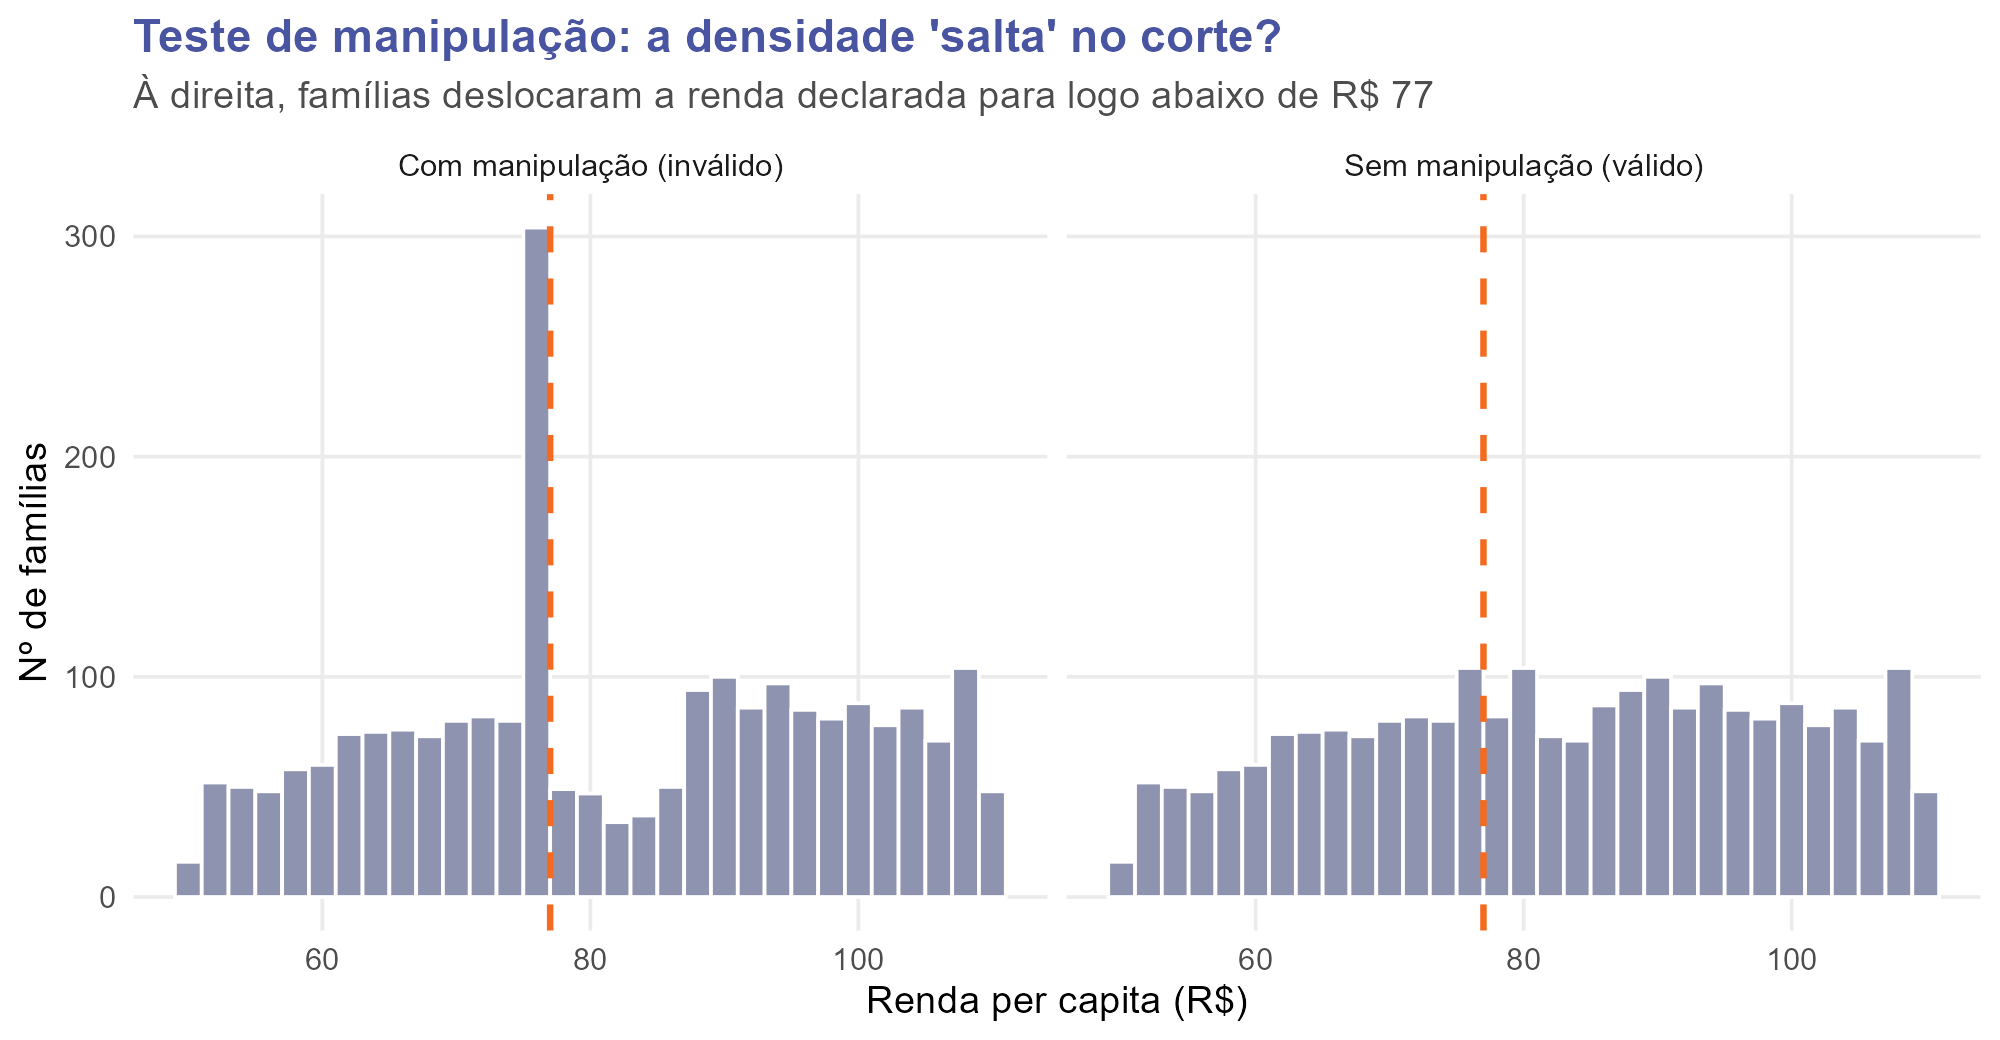
\includegraphics[height=3.7cm]{05_rdd_manipulacao.png}\par
  \footnotesize À esquerda, famílias deslocaram a renda declarada para logo abaixo de R\$ 77: o RDD perde a validade.
\end{frame}
